\documentclass[a4paper,twocolumn,12pt]{article}
\usepackage[utf8]{inputenc}
\usepackage[MeX]{polski}
\usepackage{fullpage}
\usepackage[breaklinks=true]{hyperref}
\usepackage{amsmath}
\usepackage{amssymb}
\usepackage{pgfplots}
\usepackage{subfigure}
\usepackage{textcomp}

\title{
 \LARGE{Projekt aplikacji mobilnej umożliwiającej umieszczenie wirtualnej grafiki w rzeczywistym położeniu} 
 \\ \vspace{2mm} 
 \large{Podstawy przetwarzania obrazów}
}
\author{Michał Aniserowicz}
\date{\today}

\begin{document}

\maketitle

\begin{abstract}
Celem artykułu jest opisanie zbioru koncepcji, które posłużą do implementacji algorytmu sztucznej inteligencji grającego w~grę Scrabble w~języku polskim. W~artykule zostały przeanalizowane i~porównane dane zawarte w~dwóch głównych słownikach wyrazów do gier dla języka polskiego, przedstawione dane statystyczne ułatwiające wprowadzanie heurystyk do algorytmu, a~także opisane metody niezbędne do wyznaczania wszystkich możliwych kombinacji ruchów w~danej turze. Autor omawia również podział rozgrywki na fazy gry i~przybliża podejście, które pozwala uzyskiwać najlepsze wyniki na każdym etapie rozgrywki.
\end{abstract}

\section*{Wstęp}



\section{Splot macierzy obrazów}

\begin{enumerate}
 \item Określenie:
  \begin{itemize}
   \item macierzy (maski) filtru
   \item współczynnika normalizującego (najczęściej równego sumie wartości komórek maski)
  \end{itemize}
 \item Obliczenie wartości każdego piksela obrazu poprzez:
  \begin{itemize}
   \item pomnożenie wartości komórek maski przez wartości odpowiednich piskeli,
   \item zsumowanie wartości wszystkich komórek maski
   \item podzielenie wyniku przez współczynnik normalizujący
  \end{itemize}
 \item Wartość współczynnika normalizującego równa sumie wartości komórek maski gwarantuje wartość wyniku mieszczącą się w przedziale dopuszczalnych wartości piksela (np. 0-255)
\end{enumerate}

\begin{figure}[!ht]
 \begin{center}
  \scalebox{0.25}
  {
   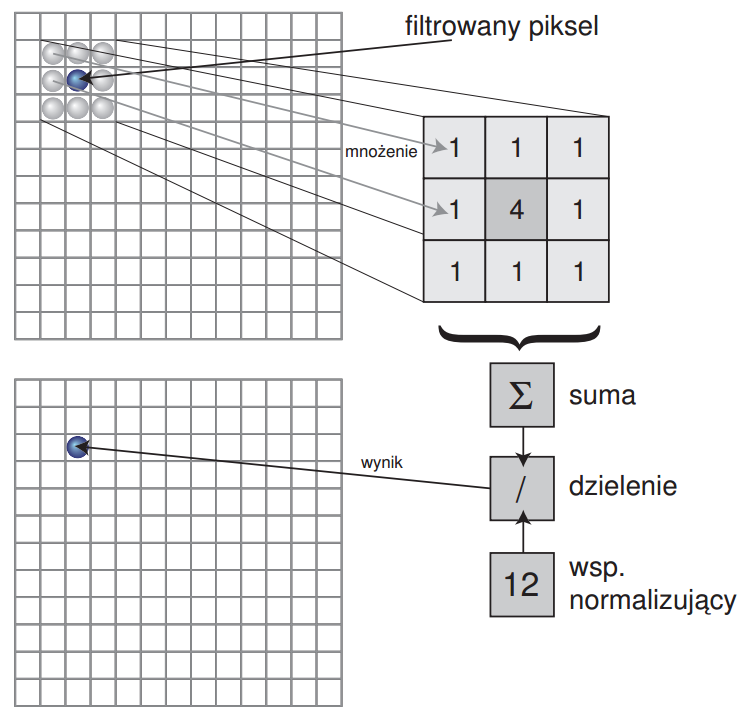
\includegraphics{../obrazki/filtry/splot.png}
  }
 \end{center}
 \caption{
  Operacja splotu.
  Źródło: TODO
 }
 \label{fig:convolution}
\end{figure}


\subsection{Przykład - rozmycie Gaussa}

\begin{itemize}
 \item Wartość piksela maleje wraz z odległością od środka
 \item Jest to filtr uśredniający
 \item Pozwala wygładzić obraz (redukując szum, ale tracąc detale)
\end{itemize}

\begin{figure}[!ht]
 \begin{center}
  \subfigure[]{
   $\begin{bmatrix}
     1 & 2 & 1 \\
     2 & 4 & 2 \\
     1 & 2 & 1
    \end{bmatrix}$
  }
  \subfigure[]{
   $\begin{bmatrix}
     1 & 1 & 2 & 1 & 1 \\
     1 & 2 & 4 & 2 & 1 \\
     2 & 4 & 8 & 4 & 2 \\
     1 & 2 & 4 & 2 & 1 \\
     1 & 1 & 2 & 1 & 1
    \end{bmatrix}$
  }
 \end{center}
 \caption{
  Maski:
  (a) 3x3;
  (b) 5x5.
 }
 \label{fig:gauss_matrices}
\end{figure}

\begin{figure}[!ht]
 \begin{center}
  \subfigure[]{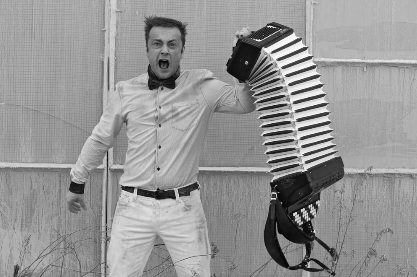
\includegraphics[width=0.33\textwidth]{../obrazki/filtry/gauss_before.jpg}}
  \subfigure[]{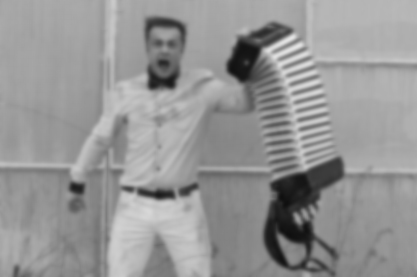
\includegraphics[width=0.33\textwidth]{../obrazki/filtry/gauss_after.jpg}}
 \end{center}
 \caption{
  Przykładowy rezultat:
  (a) przed;
  (b) po.
 }
 \label{fig:gauss_example}
\end{figure}



\section{Detekcja krawędzi}

\begin{enumerate}
 \item Zastosowanie operatorów dyskretnego różniczkowania w celu aproksymacji pochodnych kierunkowych intensywności obrazu (gradientów) w kilku kierunkach
 \item Operatory różnią się liczbą i rodzajem masek
\end{enumerate}

\begin{figure}[!ht]
 \begin{center}
  \subfigure[]{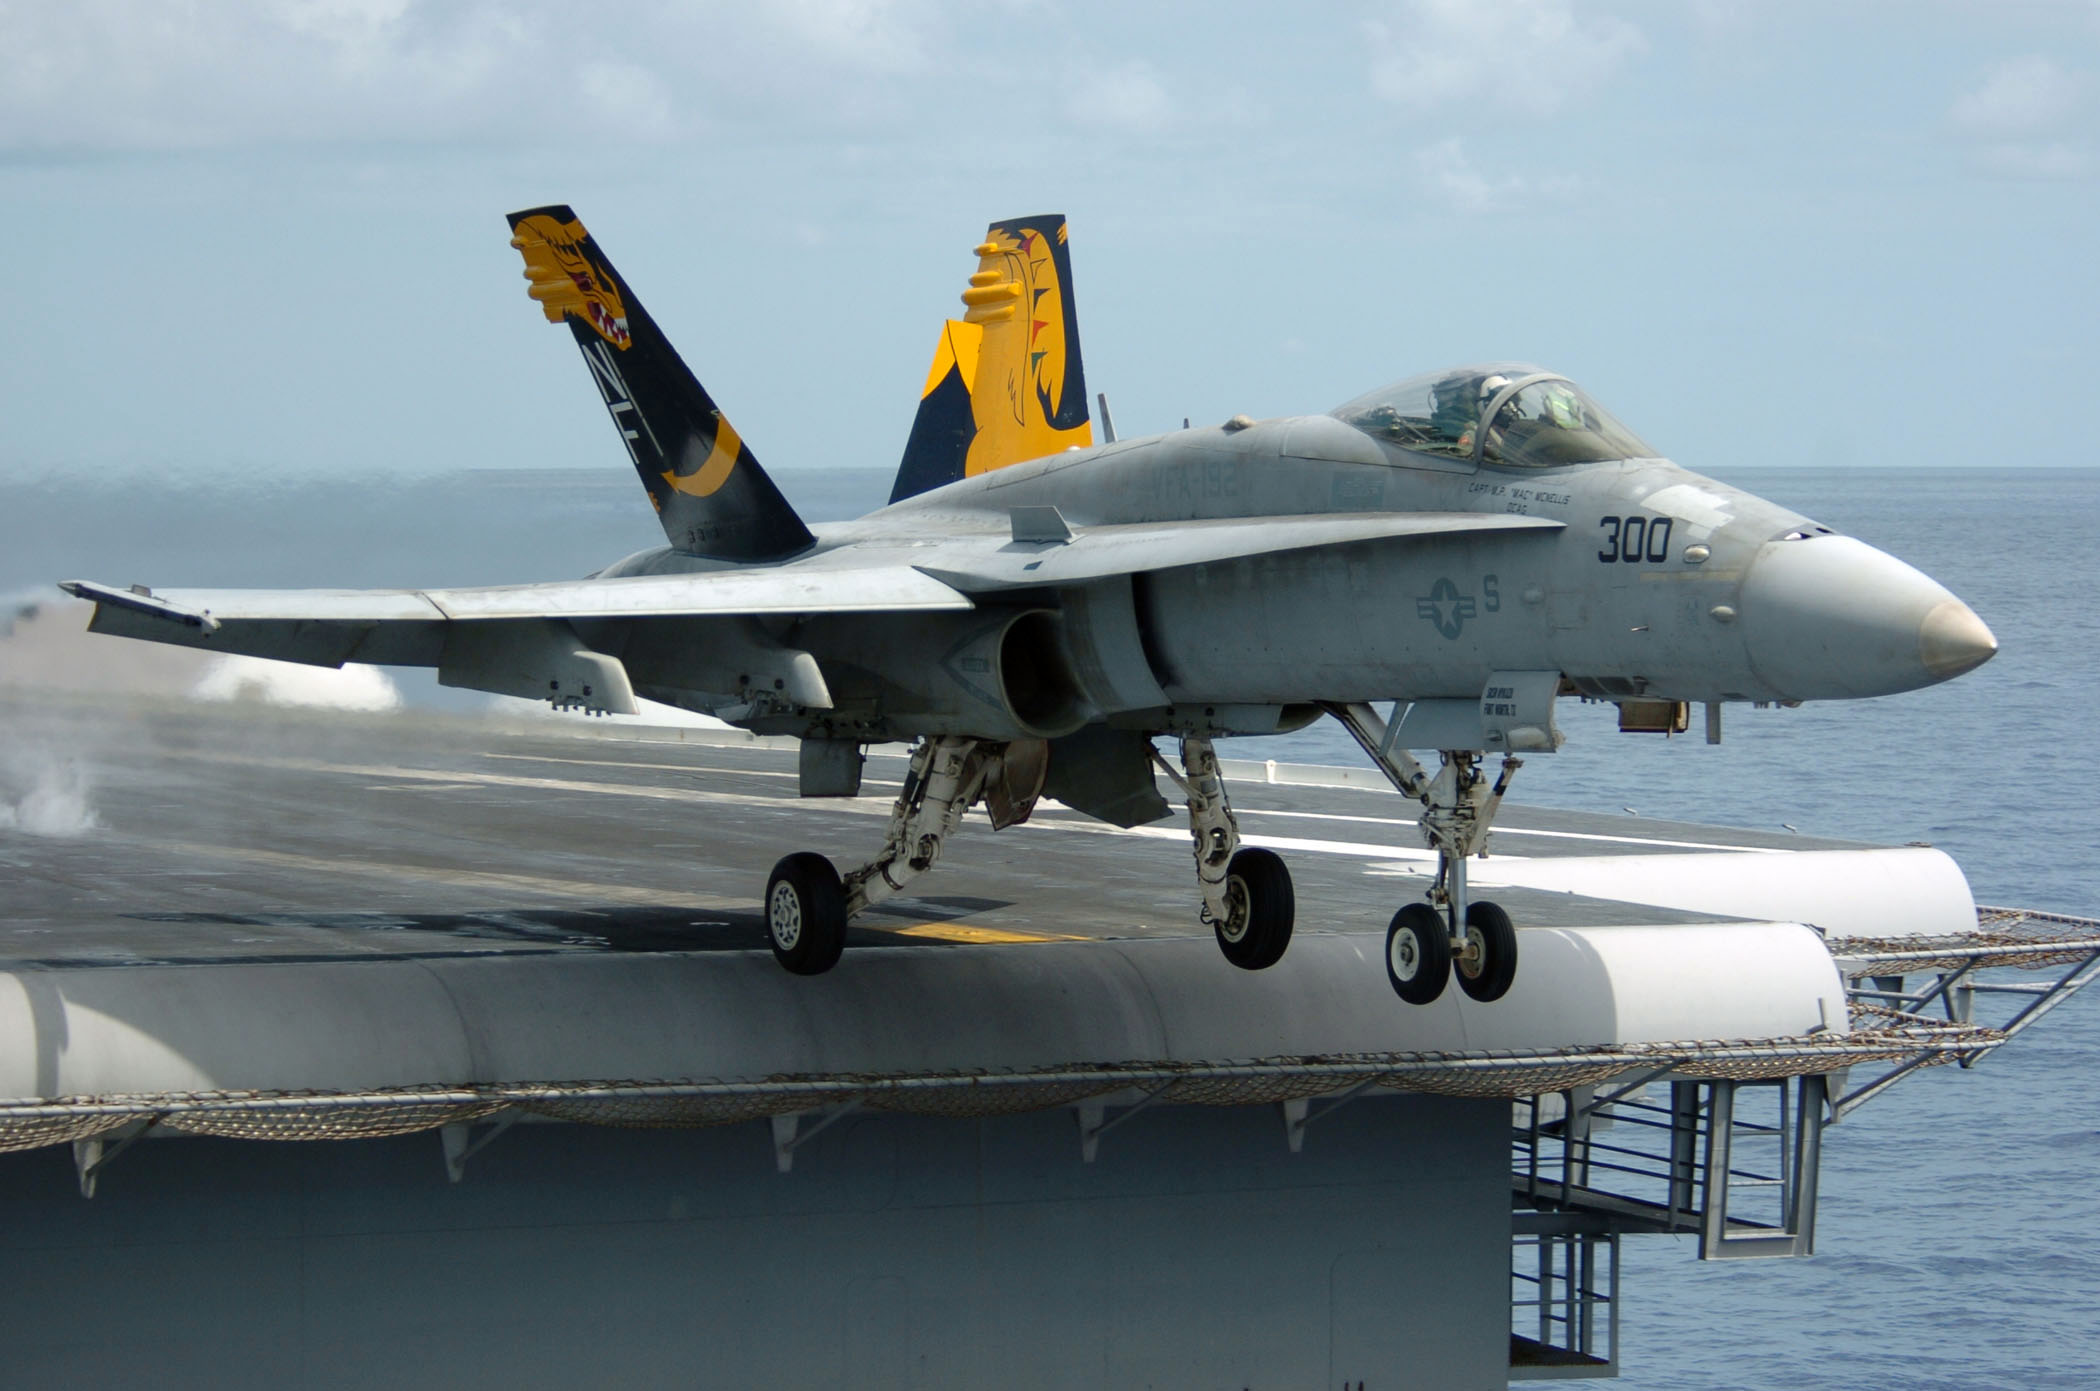
\includegraphics[width=0.33\textwidth]{../obrazki/filtry/edges_before.jpg}}
  \subfigure[]{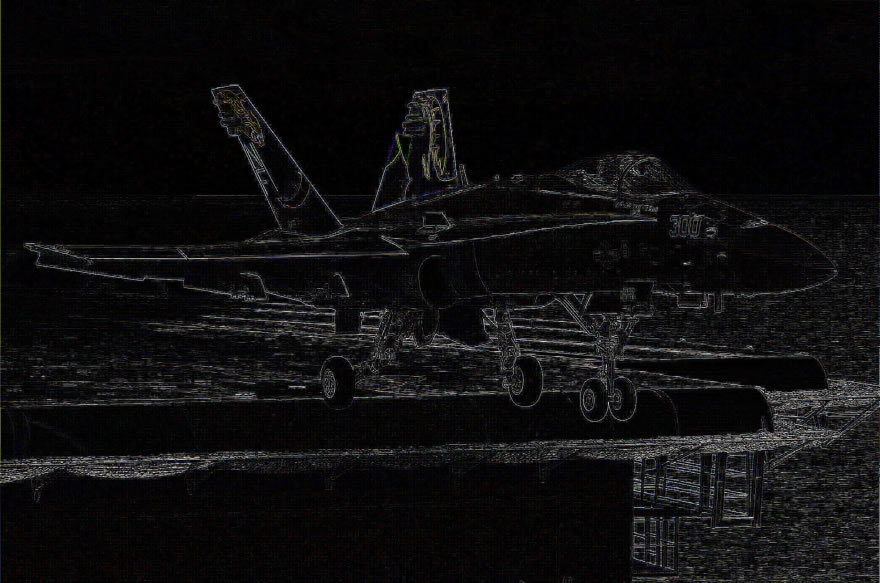
\includegraphics[width=0.33\textwidth]{../obrazki/filtry/edges_after.jpg}}
 \end{center}
 \caption{
  Przykładowy rezultat:
  (a) przed;
  (b) po.
 }
 \label{fig:edges_example}
\end{figure}


\subsection{Krzyż Robertsa}

\begin{itemize}
 \item Jeden z najwcześniejszych algorytmów wykrywania krawędzi
 \item Zaproponowany w 1963 r. przez Lawrence’a G. Robertsa
 \item Wynikowy obraz otrzymuje się poprzez obliczenie różnic modułów wartości odpowiadających sobie pikseli z obrazów powstałych przez zastosowanie masek
 \item Zaleta: mała złożoność obliczeniowa
 \item Wada: mała odporność na szum
\end{itemize}

\begin{figure}[!ht]
 \begin{center}
  \subfigure[]{
   $\begin{bmatrix}
      0 & +1 \\
     -1 &  0
    \end{bmatrix}$
  }
  \subfigure[]{
   $\begin{bmatrix}
     +1 &  0 \\
      0 & -1
    \end{bmatrix}$
  }
 \end{center}
 \caption{
  Maski:
  (a) 45\textdegree;
  (b) 135\textdegree.
 }
 \label{fig:roberts_matrices}
\end{figure}


\subsection{Prewitt}

\begin{itemize}
 \item Zaproponowany w 1966 r. przez Judith M. Prewitt
 \item Zbiór 8 masek (0\textdegree - krawędzie pionowe, 90\textdegree - poziome)
 \item Wystarczy obliczyć splot z 4 macierzami ($M_{\alpha+180^\circ} = -M_\alpha$)
 \item Lepsza skuteczność, ale większa złożoność obliczeniowa
\end{itemize}

\begin{figure}[!ht]
 \begin{center}
  \subfigure[]{
   $\begin{bmatrix}
     -1 & 0 & +1 \\
     -1 & 0 & +1 \\
     -1 & 0 & +1
    \end{bmatrix}$
  }
  \subfigure[]{
   $\begin{bmatrix}
      0 & +1 & +1 \\
     -1 &  0 & +1 \\
     -1 & -1 &  0
    \end{bmatrix}$
  }
  \subfigure[]{
   $\begin{bmatrix}
     +1 & +1 & +1 \\
      0 &  0 &  0 \\
     -1 & -1 & -1
    \end{bmatrix}$
  }
  \subfigure[]{
   $\begin{bmatrix}
     +1 & +1 &  0 \\
     +1 &  0 & -1 \\
      0 & -1 & -1
    \end{bmatrix}$
  }
 \end{center}
 \caption{
  Maski:
  (a) 0\textdegree;
  (b) 45\textdegree;
  (c) 90\textdegree;
  (d) 135\textdegree.
 }
 \label{fig:prewitt_matrices}
\end{figure}


\subsection{Sobel}

\begin{enumerate}
 \item Zaproponowany w 1968 r. przez Irwina Sobela
 \item Od operatora Prewitt różni się jedynie wagami komórek masek (1, 2, 1)
 \item Lepsze wygładzenie obrazu
\end{enumerate}

\begin{figure}[!ht]
 \begin{center}
  \subfigure[]{
   $\begin{bmatrix}
     -1 & 0 & +1 \\
     -2 & 0 & +2 \\
     -1 & 0 & +1
    \end{bmatrix}$
  }
  \subfigure[]{
   $\begin{bmatrix}
      0 & +1 & +2 \\
     -1 &  0 & +1 \\
     -2 & -1 &  0
    \end{bmatrix}$
  }
  \subfigure[]{
   $\begin{bmatrix}
     +1 & +2 & +1 \\
      0 &  0 &  0 \\
     -1 & -2 & -1
    \end{bmatrix}$
  }
  \subfigure[]{
   $\begin{bmatrix}
     +2 & +1 &  0 \\
     +1 &  0 & -1 \\
      0 & -1 & -2
    \end{bmatrix}$
  }
 \end{center}
 \caption{
  Maski:
  (a) 0\textdegree;
  (b) 45\textdegree;
  (c) 90\textdegree;
  (d) 135\textdegree.
 }
 \label{fig:sobel_matrices}
\end{figure}


\subsection{Scharr}

\begin{itemize}
 \item Zaproponowany w 2000 r. przez Hanno Scharra
 \item Od operatorów Prewitt i Sobela różni się jedynie wagami komórek masek (3, 10, 3)
 \item Lepiej wykrywa kierunek krawędzi
\end{itemize}

\begin{figure}[!ht]
 \begin{center}
  \subfigure[]{
   $\begin{bmatrix}
     -3  & 0 & +3  \\
     -10 & 0 & +10 \\
     -3  & 0 & +3
    \end{bmatrix}$
  }
  \subfigure[]{
   $\begin{bmatrix}
      0  & +3 & +10 \\
     -3  &  0 & +3  \\
     -10 & -3 &  0
    \end{bmatrix}$
  }
  \subfigure[]{
   $\begin{bmatrix}
     +3 & +10 & +3 \\
      0 &  0  &  0 \\
     -3 & -10 & -3
    \end{bmatrix}$
  }
  \subfigure[]{
   $\begin{bmatrix}
     +10 & +3 &  0 \\
     +3  &  0 & -3 \\
      0  & -3 & -10
    \end{bmatrix}$
  }
 \end{center}
 \caption{
  Maski:
  (a) 0\textdegree;
  (b) 45\textdegree;
  (c) 90\textdegree;
  (d) 135\textdegree.
 }
 \label{fig:scharr_matrices}
\end{figure}


\subsection{Porównanie}

\begin{figure}[!ht]
 \begin{center}
  \subfigure[]{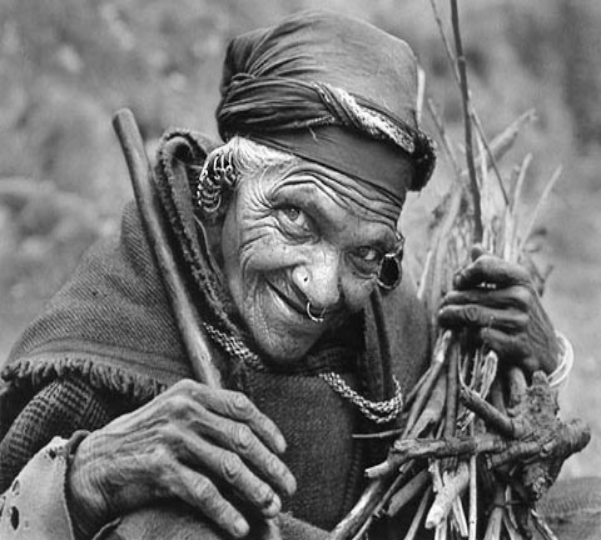
\includegraphics[width=0.33\textwidth]{../obrazki/filtry/init.png}}
  \subfigure[]{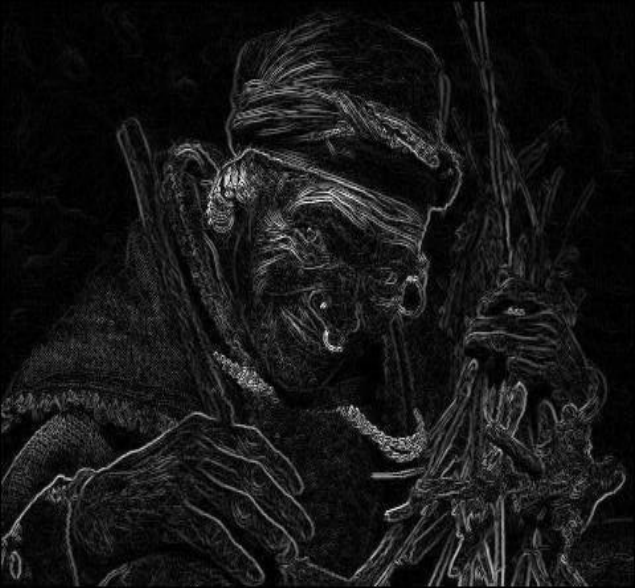
\includegraphics[width=0.33\textwidth]{../obrazki/filtry/roberts.png}}
  \subfigure[]{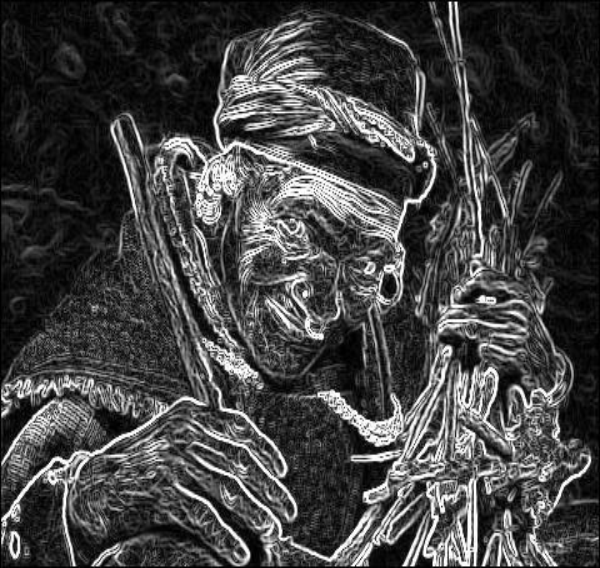
\includegraphics[width=0.33\textwidth]{../obrazki/filtry/prewitt.png}}
  \subfigure[]{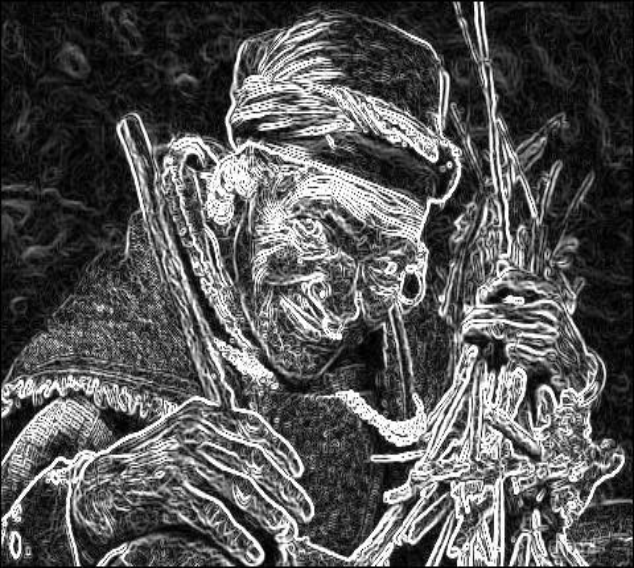
\includegraphics[width=0.33\textwidth]{../obrazki/filtry/sobel.png}}
 \end{center}
 \caption{
  Przykładowy rezultat:
  (a) przed;
  (b) Robets;
  (c) Prewitt;
  (d) Sobel.
 }
 \label{fig:edges_comparison}
\end{figure}



\section{Canny}

\begin{itemize}
 \item Autor: John F. Canny, 1986
 \item Cele:
  \begin{itemize}
   \item dobra detekcja – wykrycie jak największej liczby rzeczywistych krawędzi
   \item dobra lokalizacja – oznaczenie danej krawędzi jak najbliżej jej rzeczywistego położenia
   \item minimalna odpowiedź – oznaczenie danej krawędzi tylko raz, brak krawędzi powstałych w wyniku zakłóceń
  \end{itemize}
\end{itemize}

Kroki algorytmu:
\begin{enumerate}
 \item Wygładzenie obrazu
 \item Obliczenie modułu gradientu obrazu
 \item Usunięcie niemaksymalnych pikseli
 \item Progowanie z histerezą
\end{enumerate}


\subsection{Wygładzenie obrazu}

\begin{itemize}
 \item Wygładzenie obrazu filtrem Gaussa
 \item Odchylenie standardowe filtru ($\sigma$) - parametr metody
 \item Im większe $\sigma$, tym mniej fałszywych krawędzi
 \item Cel: redukcja szumu
\end{itemize}

\begin{figure}[!ht]
 \begin{center}
  \subfigure[]{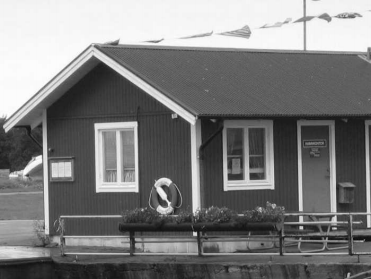
\includegraphics[width=0.33\textwidth]{../obrazki/canny/0_init.png}}
  \subfigure[]{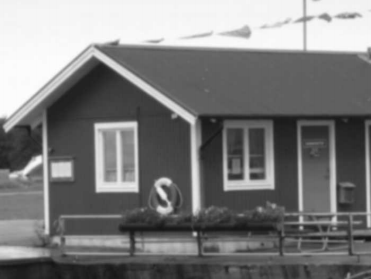
\includegraphics[width=0.33\textwidth]{../obrazki/canny/1_gauss.png}}
 \end{center}
 \caption{
  Przykładowy rezultat ($\sigma = 3$):
  (a) przed;
  (b) po.
 }
 \label{fig:canny_smoothing}
\end{figure}


\subsection{Obliczenie gradientu}

\begin{enumerate}
 \item Ponowne filtrowanie obrazu (Krzyż Robertsa / Prewitt / Sobel / Scharr)
 \item Cel: znalezienie potencjalnych krawędzi
 \item Należy zapamiętać kierunek gradientu
 \item Kierunek wyznacza się z dokładnością do 45° (pion, poziom, skosy)
\end{enumerate}

\begin{figure}[!ht]
 \begin{center}
  \subfigure[]{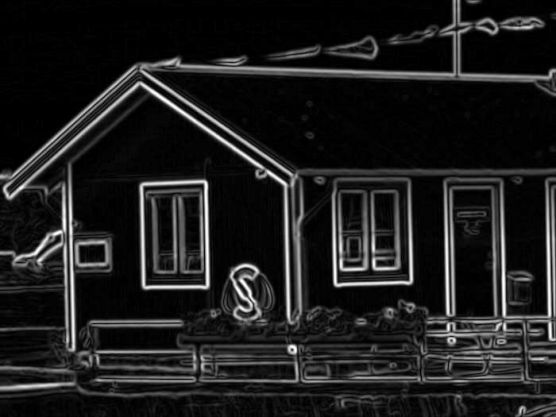
\includegraphics[width=0.33\textwidth]{../obrazki/canny/2_1_gradient.png}}
  \subfigure[]{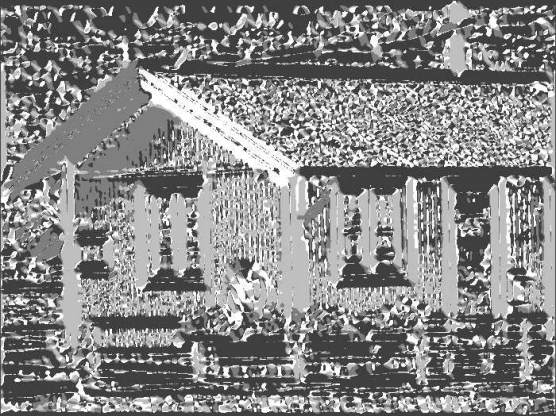
\includegraphics[width=0.33\textwidth]{../obrazki/canny/2_2_kierunek_gradientu.png}}
 \end{center}
 \caption{
  Przykładowy rezultat:
  (a) Potenscjalne krawędzie
  (b) Kierunek gradientu (ten sam odcień szarości przypisany krawędzion o tym samym nachyleniu)
 }
 \label{fig:canny_gradient}
\end{figure}


\subsection{Usunięcie zbędnych pikseli}

\begin{enumerate}
 \item Porównanie każdego pikela z dwoma pikselami sąsiednimi
 \item Piksele sąsiednie wyznaczane na podstawie informacji o kierunku gradientu
 
  \begin{figure}[!ht]
   \begin{center}
    \scalebox{0.25}
    {
     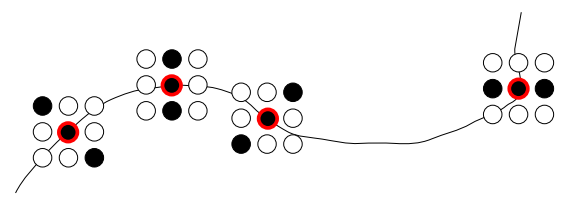
\includegraphics{../obrazki/canny/3_1_piksele.png}
    }
   \end{center}
   \caption{
    Przykład.
    Źródło: TODO
   }
   \label{fig:canny_adjacent_pixels}
  \end{figure}

 \item Jeśli jasność piksela nie jest większa od jasności obu sąsiadów, piksel ten jest zerowany
 \item Cel: uzyskanie linii o grubości 1px
 \item Pozostaje pozbyć się zbyt ciemnych krawędzi
\end{enumerate}

\begin{figure}[!ht]
 \begin{center}
  \scalebox{0.25}
  {
   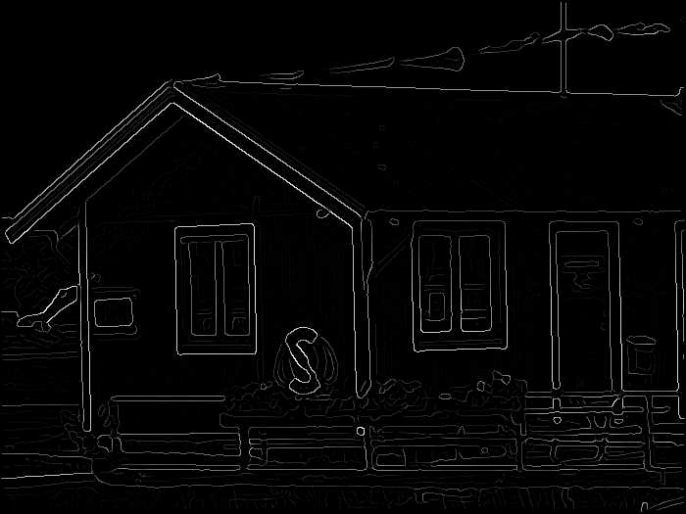
\includegraphics{../obrazki/canny/3_2_krawedzie.png}
  }
 \end{center}
 \caption{
  Przykładowy rezultat.
 }
 \label{fig:canny_redundant_pixels_removal}
\end{figure}


\subsection{Progowanie z histerezą}

\begin{enumerate}
 \item Określenie dwóch progów: $T_1$, $T_2$
 \item $T_1$, $T_2$ – parametry  metody
 \item Zaakceptowanie krawędzi, dla których moduł gradientu jest > $T_2$
 \item Usunięcie krawędzi, dla których moduł gradientu jest < $T_1$
 \item Rekurencyjne usunięcie krawędzi, dla których moduł gradientu jest < $T_2$, i które nie przylegają do już zaakceptowanej krawędzi
 \item Cel: usunięcie ciemnych krawędzi przy zachowaniu ciemnych fragmentów jasnych krawędzi
\end{enumerate}


\subsection{Przykładowe rezultaty}

\begin{figure}[!ht]
 \begin{center}
  \subfigure[]{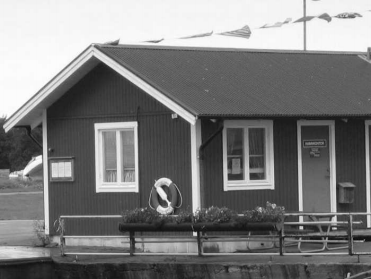
\includegraphics[width=0.33\textwidth]{../obrazki/canny/0_init.png}}
  \subfigure[]{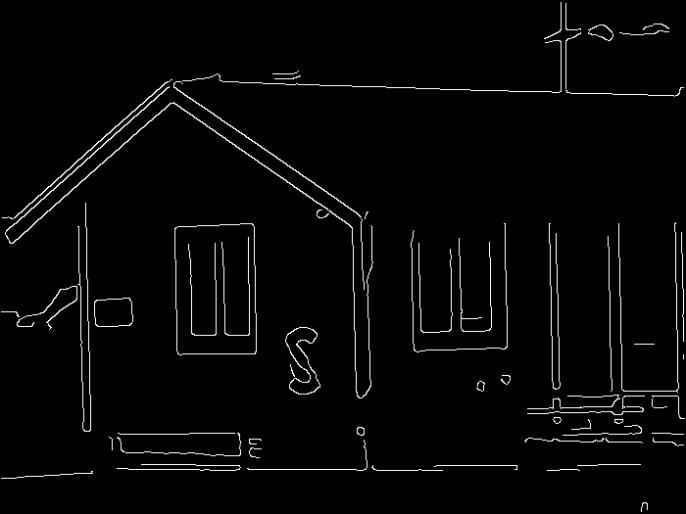
\includegraphics[width=0.33\textwidth]{../obrazki/canny/4_1_wynik_3_75_125.png}}
  \subfigure[]{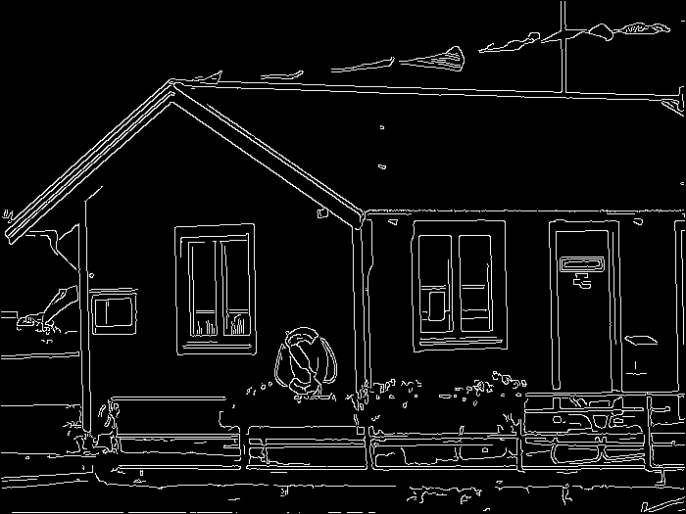
\includegraphics[width=0.33\textwidth]{../obrazki/canny/4_2_wynik_1_75_125.png}}
  \subfigure[]{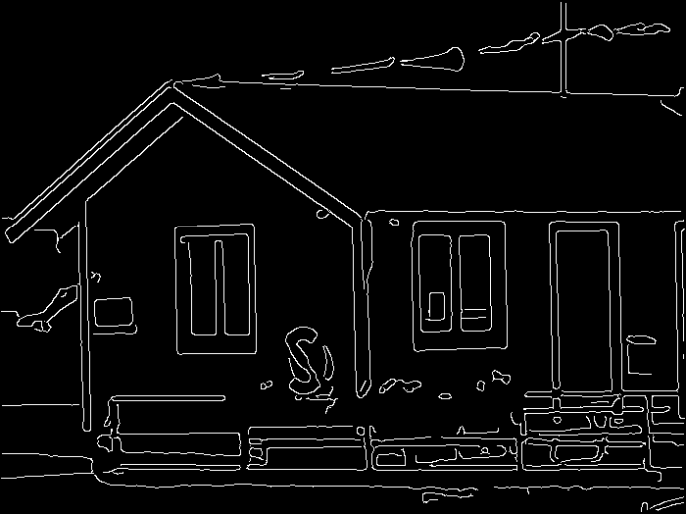
\includegraphics[width=0.33\textwidth]{../obrazki/canny/4_3_wynik_3_25_75.png}}
 \end{center}
 \caption{
  Przykładowe rezultaty:
  (a) przed;
  (b) $\sigma = 3, T_1 = 75, T_2 = 125$;
  (c) $\sigma = 1, T_1 = 75, T_2 = 125$;
  (d) $\sigma = 3, T_1 = 25, T_2 = 75$.
 }
 \label{fig:canny_comparison}
\end{figure}



\section{Podsumowanie}

\begin{itemize}
 \item Wykrywanie krawędzi (a także wiele innych operacji) sprowadza się do zastosowania dyskretnego splotu macierzy
 \item Algorytmy zaproponowane w latach 60., czy 80. są nadal stosowane
 \item Operator Sobela i algorytm Canny’ego to obecnie najpopularniejsze metody wykrywania krawędzi
\end{itemize}



\begin{thebibliography}{9}
 \small
 
 \bibitem{stec}
  \emph{Filtracja obrazów rastrowych} [online],
  Steć P.,
  http://www.uz.zgora.pl/$\sim$pstec/files/filtracja.pdf [dostęp: styczeń 2013].
  
 \bibitem{boldak}
  \emph{Wykrywanie cech w obrazach cyfrowych} [online],
  Bołdak C.,
  http://aragorn.pb.bialystok.pl/$\sim$boldak/DIP/CPO-W04-v01-50pr.pdf [dostęp: styczeń 2013].
  
 \bibitem{maini}
  \emph{Study and Comparison of Various Image Edge Detection Techniques} [online],
  Maini R., Aggarwal H.,
  http://wwwmath.tau.ac.il/$\sim$turkel/notes/Maini.pdf [dostęp: styczeń 2013].
 
 \bibitem{scrabble_definition} 
  \emph{Komputerowa analiza i przetwarzanie obrazów},
  Tadeusiewicz R., Korohoda P.,
  Kraków,
  Wydawnictwo Fundacji Postępu Telekomunikacji,
  1997,
  83-86476-15-X.
  
\end{thebibliography}

\end{document}
